%%%%%%%%%%%%%%%%%%%%%%%%%%%%%%%%%%%%%%%%%
% baposter Portrait Poster
% LaTeX Template
% Version 1.0 (15/5/13)
%
% Created by:
% Brian Amberg (baposter@brian-amberg.de)
%
% This template has been downloaded from:
% http://www.LaTeXTemplates.com
%
% License:
% CC BY-NC-SA 3.0 (http://creativecommons.org/licenses/by-nc-sa/3.0/)
%
%%%%%%%%%%%%%%%%%%%%%%%%%%%%%%%%%%%%%%%%%

%----------------------------------------------------------------------------------------
%	PACKAGES AND OTHER DOCUMENT CONFIGURATIONS
%----------------------------------------------------------------------------------------

\documentclass[a0paper,portrait,columns=2]{baposter}

\usepackage[font=small,labelfont=bf]{caption} % Required for specifying captions to tables and figures
\usepackage{booktabs} % Horizontal rules in tables
\usepackage{relsize} % Used for making text smaller in some places
\usepackage{tipa}
\usepackage{amssymb}
\usepackage{multirow}
\usepackage{multicol}
\usepackage{tikz}
\usepackage[margin=.7cm]{caption}
\usepackage{hhline}
\usepackage{colortbl}


\usetikzlibrary{arrows,decorations.pathmorphing,backgrounds,positioning,fit,matrix,trees,mindmap,shapes}

\graphicspath{{figures/}} % Directory in which figures are stored

% UA colors
% UA red	R 171	G 5	B 32
% UA blue	R 0	G 33	B 71
% UA copper	R 163	G 102	B 77

\definecolor{bordercol}{RGB}{0,33,71} % Border color of content boxes
\definecolor{headercol1}{RGB}{171,5,32} % Background color for the header in the content boxes (left side)
\definecolor{headercol2}{RGB}{171,5,32} % Background color for the header in the content boxes (right side)
\definecolor{headerfontcol}{RGB}{255,255,255} % Text color for the header text in the content boxes
\definecolor{boxcolor}{RGB}{255,255,255} % Background color for the content in the content boxes
\definecolor{uared}{RGB}{204,0,51}

\usepackage{enumitem}
\setlist{nolistsep}


\begin{document}


\background{ % Set the background to an image (background.pdf)
\begin{tikzpicture}[remember picture,overlay]
\draw (current page.north west)+(-2em,2em) node[anchor=north west]
{
\includegraphics[height=1.1\textheight]{bg}};
\end{tikzpicture}
}

\begin{poster}{
grid=false,
borderColor=bordercol, % Border color of content boxes
headerColorOne=headercol1, % Background color for the header in the content boxes (left side)
headerColorTwo=headercol2, % Background color for the header in the content boxes (right side)
headerFontColor=headerfontcol, % Text color for the header text in the content boxes
boxColorOne=boxcolor, % Background color for the content in the content boxes
headershape=roundedright, % Specify the rounded corner in the content box headers
headerfont=\Large\sf\bf, % Font modifiers for the text in the content box headers
textborder=rectangle,
background=user,
headerborder=closed, % Change to closed for a line under the content box headers
boxshade=plain
}
{}
%
%----------------------------------------------------------------------------------------
%	TITLE AND AUTHOR NAME
%----------------------------------------------------------------------------------------
%
{\sf\bf \LARGE{The effects of stress/accent on VOT depend on language (English, Spanish), consonant (/d/, /t/) and linguistic experience (monolinguals, bilinguals)}}
{\vspace{.6em} \textbf{Miquel Simonet}, \textbf{Joseph V. Casillas}, \textbf{Yamile D\'iaz}\\ 
\smaller{University of Arizona \\ Tucson, Arizona, U.S.A.} \\
{\hspace{-7in}
\includegraphics[scale=0.2]{UA_logo}\phantom{.}} \\
{\vspace{-.4in}\smaller \{simonet, jvcasill, ydiaz44\}@email.arizona.edu} \\
{\vspace{-.45in}\phantom{.}\hspace{7in}
\includegraphics[scale=0.35]{aalp_logo}}\vspace{-.6in}}




%----------------------------------------------------------------------------------------
%	INTRODUCTION
%----------------------------------------------------------------------------------------

\headerbox{Introduction}{name=introduction,column=0,row=.05}{

\vspace{.1in}

\textbf{English vs. Spanish /p t k b d g/:}

\vspace{.05in}

\begin{itemize} 
	\item English and Spanish contrast \emph{fortis} with \emph{lenis} stops
	\item One acoustic correlate of contrast is VOT
\end{itemize}

\begin{center}
	\begin{tabular}{@{}cccc@{}}
	\hline
	        & Lead & Short-lag & Long-lag \\	
	\hline
	English &      & bdg       & ptk \\
	Spanish & bdg  & ptk       & \\
	\hline
	\end{tabular}
\end{center}

\begin{itemize} 
	\item English uses [spread glottis] while Spanish uses [voice].
\end{itemize}

\vspace{.1in}

\textbf{Stress effects on VOT:}

\vspace{.05in}

\begin{itemize} 
	\item For English \emph{fortis} stops, stress \emph{lengthens} long-lag VOT \\ (Lisker \& Abramson, 1967; among others)
	\item Effects not straightforward for English \emph{lenis} stops:
	\begin{itemize}
		\item Stress \emph{shortens} VOT {\footnotesize{\cite{Abramson:1967fk}}}
		\item Stress \emph{lengthens} VOT {\footnotesize{\cite{Cole:2003uq}}}
		\item Effects small compared to \emph{fortis} stops
	\end{itemize} 
	\item Studies of Spanish stops do not examine stress effects
	\item Other languages: Stress lengthens short-lag VOT of Dutch /t/
\end{itemize} 

\vspace{.1in}

\textbf{Present study:}

\vspace{.05in}

\begin{itemize} 
	\item Consider the literature on speech rate effects on VOT:

\begin{center}
	\begin{tabular}{@{}lcccc@{}}
	\hline
	        & Lead & \cellcolor{gray!15} Short-lag                      & Long-lag                       & Reference\\
	\hline
	English &      & \cellcolor{gray!15}\textipa{t} & \textipa{t\textsuperscript{h}} & \footnotesize{\cite{kessinger1997vot}} \\
	French  & d    & \cellcolor{gray!15}t           &                                & \footnotesize{\cite{kessinger1997vot}}\\
	Thai    & d    & \cellcolor{gray!15}t           & \textipa{t\textsuperscript{h}} & \footnotesize{\cite{kessinger1997vot}} \\
	Swedish & d    & \cellcolor{gray!15}            & \textipa{t\textsuperscript{h}} & \footnotesize{\cite{beckman2011rate}} \\
	\hline
	\end{tabular}
\end{center}
% color 1st column and 3rd column

	\begin{itemize}
		\item Speech rate affects `marked' or `specified' consonants
	\end{itemize}
	\item Present study examines effects of stress on:
\end{itemize}

\begin{center}
	\begin{tabular}{@{}lcc@{}}
	\hline
	English         &         & [spread glottis] \\
	Spanish         & \phantom{....}[voice]\phantom{....} & \\
	Spanish-English & \phantom{....}[voice]\phantom{....} & [spread glottis]\\
	\hline
	\end{tabular}
\end{center}

\vspace{.05in}
}


%----------------------------------------------------------------------------------------
%	MATERIALS AND METHODS
%----------------------------------------------------------------------------------------

\headerbox{Method}{name=methods,column=0,below=introduction}{

\vspace{.1in}
\textbf{Materials}
\vspace{.05in}
\begin{itemize}
	\item Word-initial \textbf{consonant} (/d t/) $\times$ \textbf{Language} (English, Spanish) $\times$ \textbf{Stress} (stressed, unstressed) \textipa{[\textprimstress $\sigma$.$\sigma$] vs. [$\sigma$.\textprimstress$\sigma$]} \\ 5 items $\times$ 2 $\times$ 2 $\times$ 2 = 40 words
	\item Auditory stimuli. 6 `talkers' (3 Eng., 3 Sp.) each word produced 3 times. 40 words $\times$ 3 iterations = 120 different stimuli.
\end{itemize}

\vspace{.1in}
\textbf{Speakers} (N = 47) 
\vspace{-.05in}
\begin{center}
	\begin{tabular}{ll}
	Spanish monolingual   (Majorca, Spain) & N = 22 \\
	English monolingual   (Arizona, US) & N = 7 \\
	Spanish-English bilingual   (Arizona, US) & N = 19 \\
	\end{tabular}
\end{center}

\textbf{Procedure}
\vspace{.05in}
	\begin{itemize}
		\item Delayed repetition ``--is the word'' ``--es la palabra''
	\end{itemize}
	\vspace{-.05in}
		\begin{center}
			\begin{tabular}{ll}
			Spanish monolingual & Spanish block  \\
			English monolingual &  English block \\
			Spanish-English bilinguals   & Spanish/English block \\
			\end{tabular}
		\end{center}

\textbf{Analysis}
\vspace{.05in}
\begin{itemize}
	\item 4,020 tokens (420 English, 1,320 Spanish, 2,280 bilingual)
\end{itemize}
\vspace{-.2in}
\begin{center}	
	
\includegraphics[width=1.05\textwidth]{praat2.png}
\end{center}

}






%----------------------------------------------------------------------------------------
%	RESULTS
%----------------------------------------------------------------------------------------

\headerbox{Results}{name=results,column=1,row=.05}{ % To reduce this block to 1 column width, remove 'span=2'

\vspace{.1in}

\begin{center}
\vspace{.1in}
\begin{tabular}{@{}lcclcc@{}}
\hline \\ [-2ex]
\multirow{2}{*}{\textcolor{uared}{\textbf{Monolinguals}}} & \multicolumn{2}{c}{Spanish} &  & \multicolumn{2}{c}{English} \\ [.5ex]
           & /d/          & \cellcolor{gray!15}/t/          &  & \cellcolor{gray!15} /d/         & /t/ \\ [.5ex]
\hhline{~--~--} \\ [-2ex]
stressed   & -70.2 (14.7)  & 14.6 (4.4)  &  & 23.1 (7.6)  & 76.1 (16.6)\\  [1ex]
unstressed & -53.7 (14.4)  & 15.8 (5.5)  &  & 25.7 (10.3) & 69.3 (16.3)\\ [.5ex]
\hhline{~--~--} \\ [-2ex]
effect     &  16.5 \checkmark        & NS         &  & NS         & 6.8 \checkmark \\ [.5ex]
           &               &             & &            &               \\[1ex]
\hline \\ [-2ex]
\multirow{2}{*}{\textcolor{uared}{\textbf{Bilinguals}}} & \multicolumn{2}{c}{Spanish}& & \multicolumn{2}{c}{English} \\ [.5ex]
           & /d/          & \cellcolor{gray!15} /t/         & & /d/         & /t/ \\ [.5ex]
\hhline{~--~--} \\ [-2ex]
stressed   & -73.3 (36.6) & 12.2 (3.5)  & & 19.5 (3.8)  & 69.1 (19.0)\\ [1ex]
unstressed & -43.7 (41.4) & 13.2 (3.3)  & & 16.7 (14.8) & 62.3 (13.3)\\ [1ex]
\hhline{~--~--} \\ [-2ex]
effect     & 29.6 \checkmark & NS         & & 2.8 \checkmark & 6.8 \checkmark \\ 
\end{tabular}
\end{center}

\vspace{.1in}

\begin{center}
	\begin{tabular}{@{}llcrr@{}}
	\hline \\ [-2ex]
	Group          & Language & & \multicolumn{2}{c}{Stress effects} \\ [.5ex]
	\hline \\ [-2ex]
	Spanish        & Spanish  & & d \checkmark & t \phantom{\checkmark}\\ [.5ex]
	English        & English  & & d \phantom{\checkmark} & t \checkmark \\ [.5ex]
	Bilinguals     & Spanish  & & d \checkmark & t \phantom{\checkmark} \\ [.5ex]
	               & English  & & d \checkmark & t \checkmark \\ [.5ex]
	\hline
	\end{tabular}
\end{center}

\begin{center}
\captionof{figure}{Effects of lexical stress on VOT in Spanish (left) and English (right) /t/ and /d/ in the \textbf{bilingual} productions.}
\vspace{.07in}
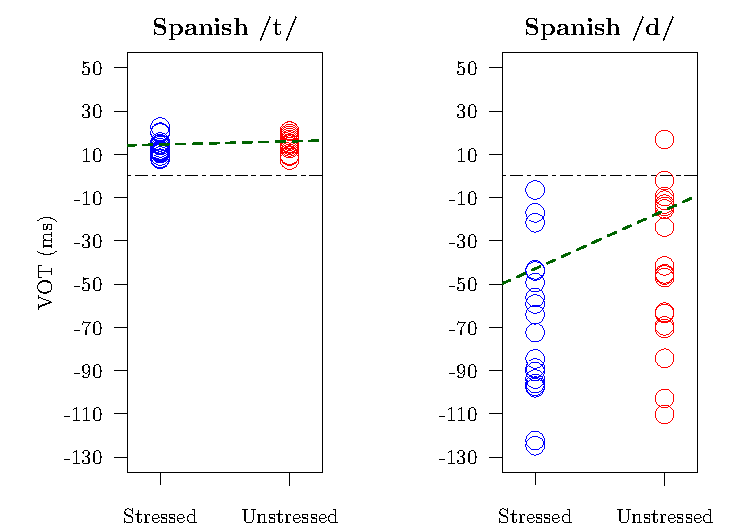
\includegraphics[width=0.45\linewidth]{bil_sp.pdf}
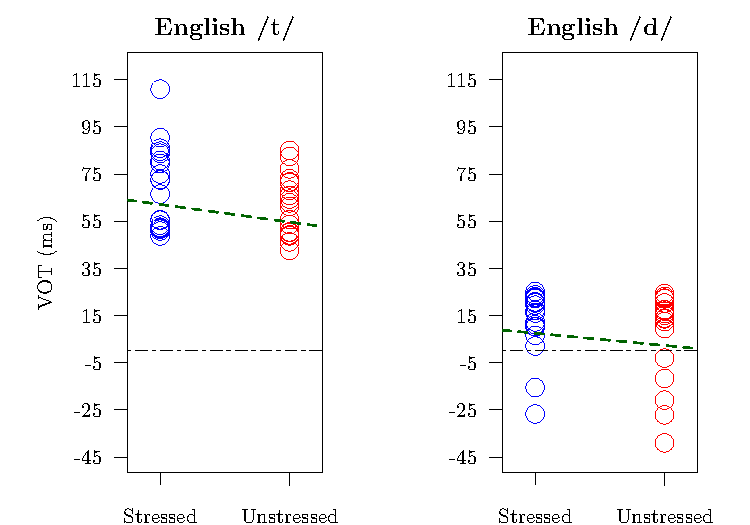
\includegraphics[width=0.45\linewidth]{bil_eng.pdf}
\end{center}

\vspace{.07in}

%------------------------------------------------


}

%----------------------------------------------------------------------------------------
%	CONCLUSION
%----------------------------------------------------------------------------------------

\headerbox{Conclusion}{name=conclusion,column=1,below=results}{

\vspace{.1in}
\textbf{Summary}
\vspace{.05in}
\begin{itemize}
	\item Spanish: stress affects /d/, but not /t/ (anchor is /t/)
	\item English: stress affects /t/, but not /d/ (anchor is /d/)
	\item Bilinguals:
	\begin{itemize}
		\item Stress affects all but Spanish /t/ (anchor is Spanish /t/)
		\item Sp. /d/ (-58) : Sp. /t/ (12) : En. /d/ (18) : En. /t/ (65)
	\end{itemize}
\end{itemize}

\vspace{.1in}

\textbf{Conclusion}
\vspace{.05in}
\begin{itemize}
	\item One anchor per individual system
	\item Anchor is category closest to VOT of 0
	\item Strict featural account of stress effects not adequate \cite{beckman2011rate}
\end{itemize}

\vspace{.03in}
}

%----------------------------------------------------------------------------------------






%----------------------------------------------------------------------------------------
%	REFERENCES
%----------------------------------------------------------------------------------------

\headerbox{Selected references}{name=references,column=1,below=conclusion}{
{\footnotesize
\smaller % Reduce the font size in this block
\renewcommand{\section}[2]{\vskip 0.05em} % Get rid of the default "References" section title
% \nocite{*} % Insert publications even if they are not cited in the poster

\bibliographystyle{unsrt}
\bibliography{IEEEabrv,SpeePros} % Use sample.bib as the bibliography file
\vspace{.02in}
}
}

%----------------------------------------------------------------------------------------
%	ACKNOWLEDGEMENTS
%----------------------------------------------------------------------------------------

% \headerbox{Acknowledgements}{name=acknowledgements,column=0,below=references, above=bottom}{

% \smaller % Reduce the font size in this block
% None.
% } 



\end{poster}

\end{document}